%%%%%%%%%%%%%%%%%%%%%%%%%%%%%%%%%%%%%%%%%
% baposter Landscape Poster
% LaTeX Template
% Version 1.0 (11/06/13)
%
% baposter Class Created by:
% Brian Amberg (baposter@brian-amberg.de)
%
% This template has been downloaded from:
% http://www.LaTeXTemplates.com
%
% License:
% CC BY-NC-SA 3.0 (http://creativecommons.org/licenses/by-nc-sa/3.0/)
%
%%%%%%%%%%%%%%%%%%%%%%%%%%%%%%%%%%%%%%%%%

%----------------------------------------------------------------------------------------
%	PACKAGES AND OTHER DOCUMENT CONFIGURATIONS
%----------------------------------------------------------------------------------------

\documentclass[portrait,a0paper,fontscale=0.285]{baposter} % Adjust the font scale/size here

\usepackage{graphicx} % Required for including images
\graphicspath{{figures/}} % Directory in which figures are stored

\usepackage{amsmath} % For typesetting math
\usepackage{amssymb} % Adds new symbols to be used in math mode

\usepackage{booktabs} % Top and bottom rules for tables
\usepackage{enumitem} % Used to reduce itemize/enumerate spacing
\usepackage{palatino} % Use the Palatino font
\usepackage[font=small,labelfont=bf]{caption} % Required for specifying captions to tables and figures

\usepackage{multicol} % Required for multiple columns
\setlength{\columnsep}{1.5em} % Slightly increase the space between columns
\setlength{\columnseprule}{0mm} % No horizontal rule between columns

\usepackage{tikz} % Required for flow chart
\usetikzlibrary{shapes,arrows} % Tikz libraries required for the flow chart in the template

\newcommand{\compresslist}{ % Define a command to reduce spacing within itemize/enumerate environments, this is used right after \begin{itemize} or \begin{enumerate}
\setlength{\itemsep}{1pt}
\setlength{\parskip}{0pt}
\setlength{\parsep}{0pt}
}



\definecolor{lightgreen}{RGB}{113,227,159} % Defines the color used for content box headers
\definecolor{lightpurp}{RGB}{171,193,180}

\begin{document}

\begin{poster}
{
headerborder=closed, % Adds a border around the header of content boxes
colspacing=1em, % Column spacing
bgColorOne=white, % Background color for the gradient on the left side of the poster
bgColorTwo=white, % Background color for the gradient on the right side of the poster
borderColor=lightgreen, % Border color
headerColorOne=lightgreen, % Background color for the header in the content boxes (left side)
headerColorTwo=lightpurp, % Background color for the header in the content boxes (right side)
headerFontColor=white, % Text color for the header text in the content boxes
boxColorOne=white, % Background color of the content boxes
textborder=rectangle, % Format of the border around content boxes, can be: none, bars, coils, triangles, rectangle, rounded, roundedsmall, roundedright or faded
eyecatcher=true, % Set to false for ignoring the left logo in the title and move the title left
headerheight=0.16\textheight, % Height of the header
headershape=rectangle, % Specify the rounded corner in the content box headers, can be: rectangle, small-rounded, roundedright, roundedleft or rounded
headerfont=\Large\bf\textsc, % Large, bold and sans serif font in the headers of content boxes
%textfont={\setlength{\parindent}{1.5em}}, % Uncomment for paragraph indentation
linewidth=1pt % Width of the border lines around content boxes
}
%----------------------------------------------------------------------------------------
%	TITLE SECTION 
%----------------------------------------------------------------------------------------
%
{
\includegraphics[height=3em]{nispero.png}} % First university/lab logo on the left
%{}
{\bf{Nispero: a cloud-computing based Scala tool specially suited for bioinformatics data
processing}}
 % Poster title
{\textsc{Evdokim~Kovach, Alexey~Alekhin, Marina~Manrique, Pablo~Pareja-Tobes, Eduardo~Pareja, Raquel~Tobes and Eduardo~Pareja-Tobes}} % Author names and institution
{
\includegraphics[height=3em]{era7.png}} % Second university/lab logo on the right


%----------------------------------------------------------------------------------------
%	OBJECTIVES
%----------------------------------------------------------------------------------------

%\headerbox{Objectives}{name=objectives,column=0,row=0}{
%uuuuuuuuuuuuuuuuuu
%}

%----------------------------------------------------------------------------------------
%	INTRODUCTION
%----------------------------------------------------------------------------------------

\headerbox{Introduction}{name=introduction,column=0,row=0}{

Nispero is a Scala library for declaring stateless computations and scaling them 
using cloud computing, in particular a combination of services from AWS
(Amazon Web Services).
}

%----------------------------------------------------------------------------------------
%	RESULTS 1
%----------------------------------------------------------------------------------------

\headerbox{Why AWS?}{name=whyaws,column=1,row=0}{
\begin{itemize}\compresslist
	\item Hire as much resources as you want
	\item pay-as-you-go
\end{itemize}
}

\headerbox{Why Scala?}{name=whyscala,column=2,row=0}{
\begin{itemize}\compresslist
	\item Type safety
	\item Java compatibility
\end{itemize}
}

\headerbox{Architecture}{name=architecture,column=1,span=2,below=whyaws}{



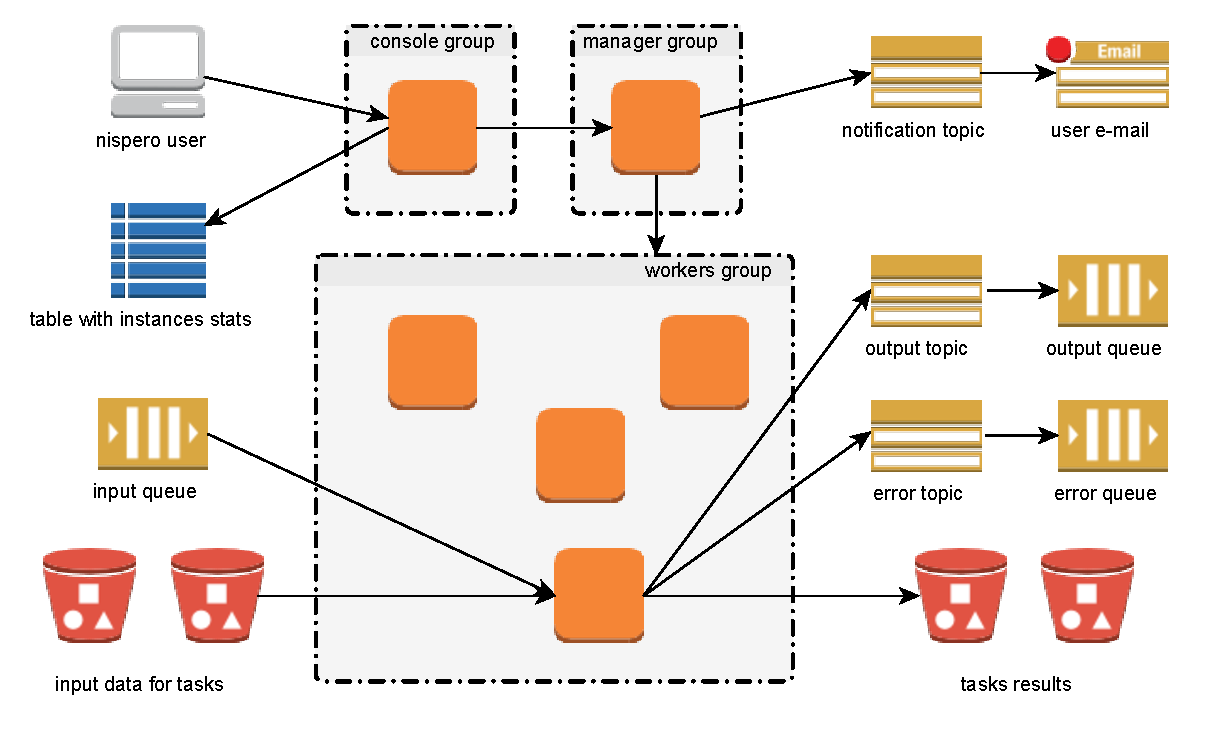
\includegraphics[width=\textwidth]{architecture.pdf}


}


%----------------------------------------------------------------------------------------
%	REFERENCES
%----------------------------------------------------------------------------------------

\headerbox{INTERCROSSING}{name=intercrossing,column=0,above=bottom}{

% \begin{columns}[T]
% 	\begin{column}{.5\textwidth}
% 		
\includegraphics[width=\textwidth]{intercrossing.png}
% 	\end{column}
% 	\begin{column}{.5\textwidth}
% 	  This project is funded in part by the ITN FP7 project INTERCROSSING (Grant 289974). 
% 	\end{column}
% \end{columns}

This project is funded in part by the ITN FP7 project INTERCROSSING (Grant 289974). \\

\hspace*{+0.4cm}
\includegraphics[width=0.3\textwidth]{intercrossing.png}
\hspace{0.20\textwidth}

\includegraphics[width=0.3\textwidth]{mc.jpg}

}




%----------------------------------------------------------------------------------------
%	FUTURE RESEARCH
%----------------------------------------------------------------------------------------


%----------------------------------------------------------------------------------------
%	CONTACT INFORMATION
%----------------------------------------------------------------------------------------

\headerbox{Availability}{name=availability,column=1,span=2,above=bottom}{ % This block is as tall as the references block



\begin{multicols}{2}



Nispero is an open-source project released under the AGPLv3 license. 
\\
The source code is available at 
\\
https://github.com/ohnosequences/nispero
\hspace*{+0.5cm}
\includegraphics[width=0.25\textwidth]{agpl.pdf}
\hspace*{+0.5cm}
\includegraphics[width=0.13\textwidth]{qrcode.pdf}

\end{multicols}


}


\headerbox{Features}{name=features,column=0,below=introduction}{ % This block's bottom aligns with the bottom of the conclusion block
\begin{itemize}\compresslist
\item For all configuration of Nispero we are using Scala, it makes possible to check it statically before any Amazon instance
will be launched
\item Nispero specially designed for bioinformatics data processing, for example it has built-in tools for working with FASTQ files. 
 \end{itemize}

%  \begin{itemize}\compresslist
%   \item Strongly typed configuration based on Scala code
%   \item CRDT-like semantics (a nispero instance is essentially a morphism 
% between idempotent commutative monoids)
%   \item Ability to run arbitrary code/programs
%   \item Automatic deploy/undeploy
%   \item Build-in FASTQ splitters.
% \end{itemize}


}

\headerbox{Applications}{name=applications,column=0,below=features}{ % This block's bottom aligns with the bottom of the conclusion block

Nispero is used as a core component of metapasta --- microbial community profiling cloud tool. 
}

\headerbox{Instructions}{name=instructions,column=0,below=applications}{ % This block's bottom aligns with the bottom of the conclusion block
Instructions represent computations that will be launched by Nispero. They can be: 
 \begin{itemize}\compresslist
  \item Scala/Java/other JVM code that implements the special interface
  \item Any BASH script following simple conventions. It makes possible to use any programming language with Nispero.
  \end{itemize}

  The input data for instructions is called a task.
}




\headerbox{Why nispero? It's tasty!}{name=whynispero,column=0,below=instructions}{ % This block's bottom aligns with the bottom of the conclusion block
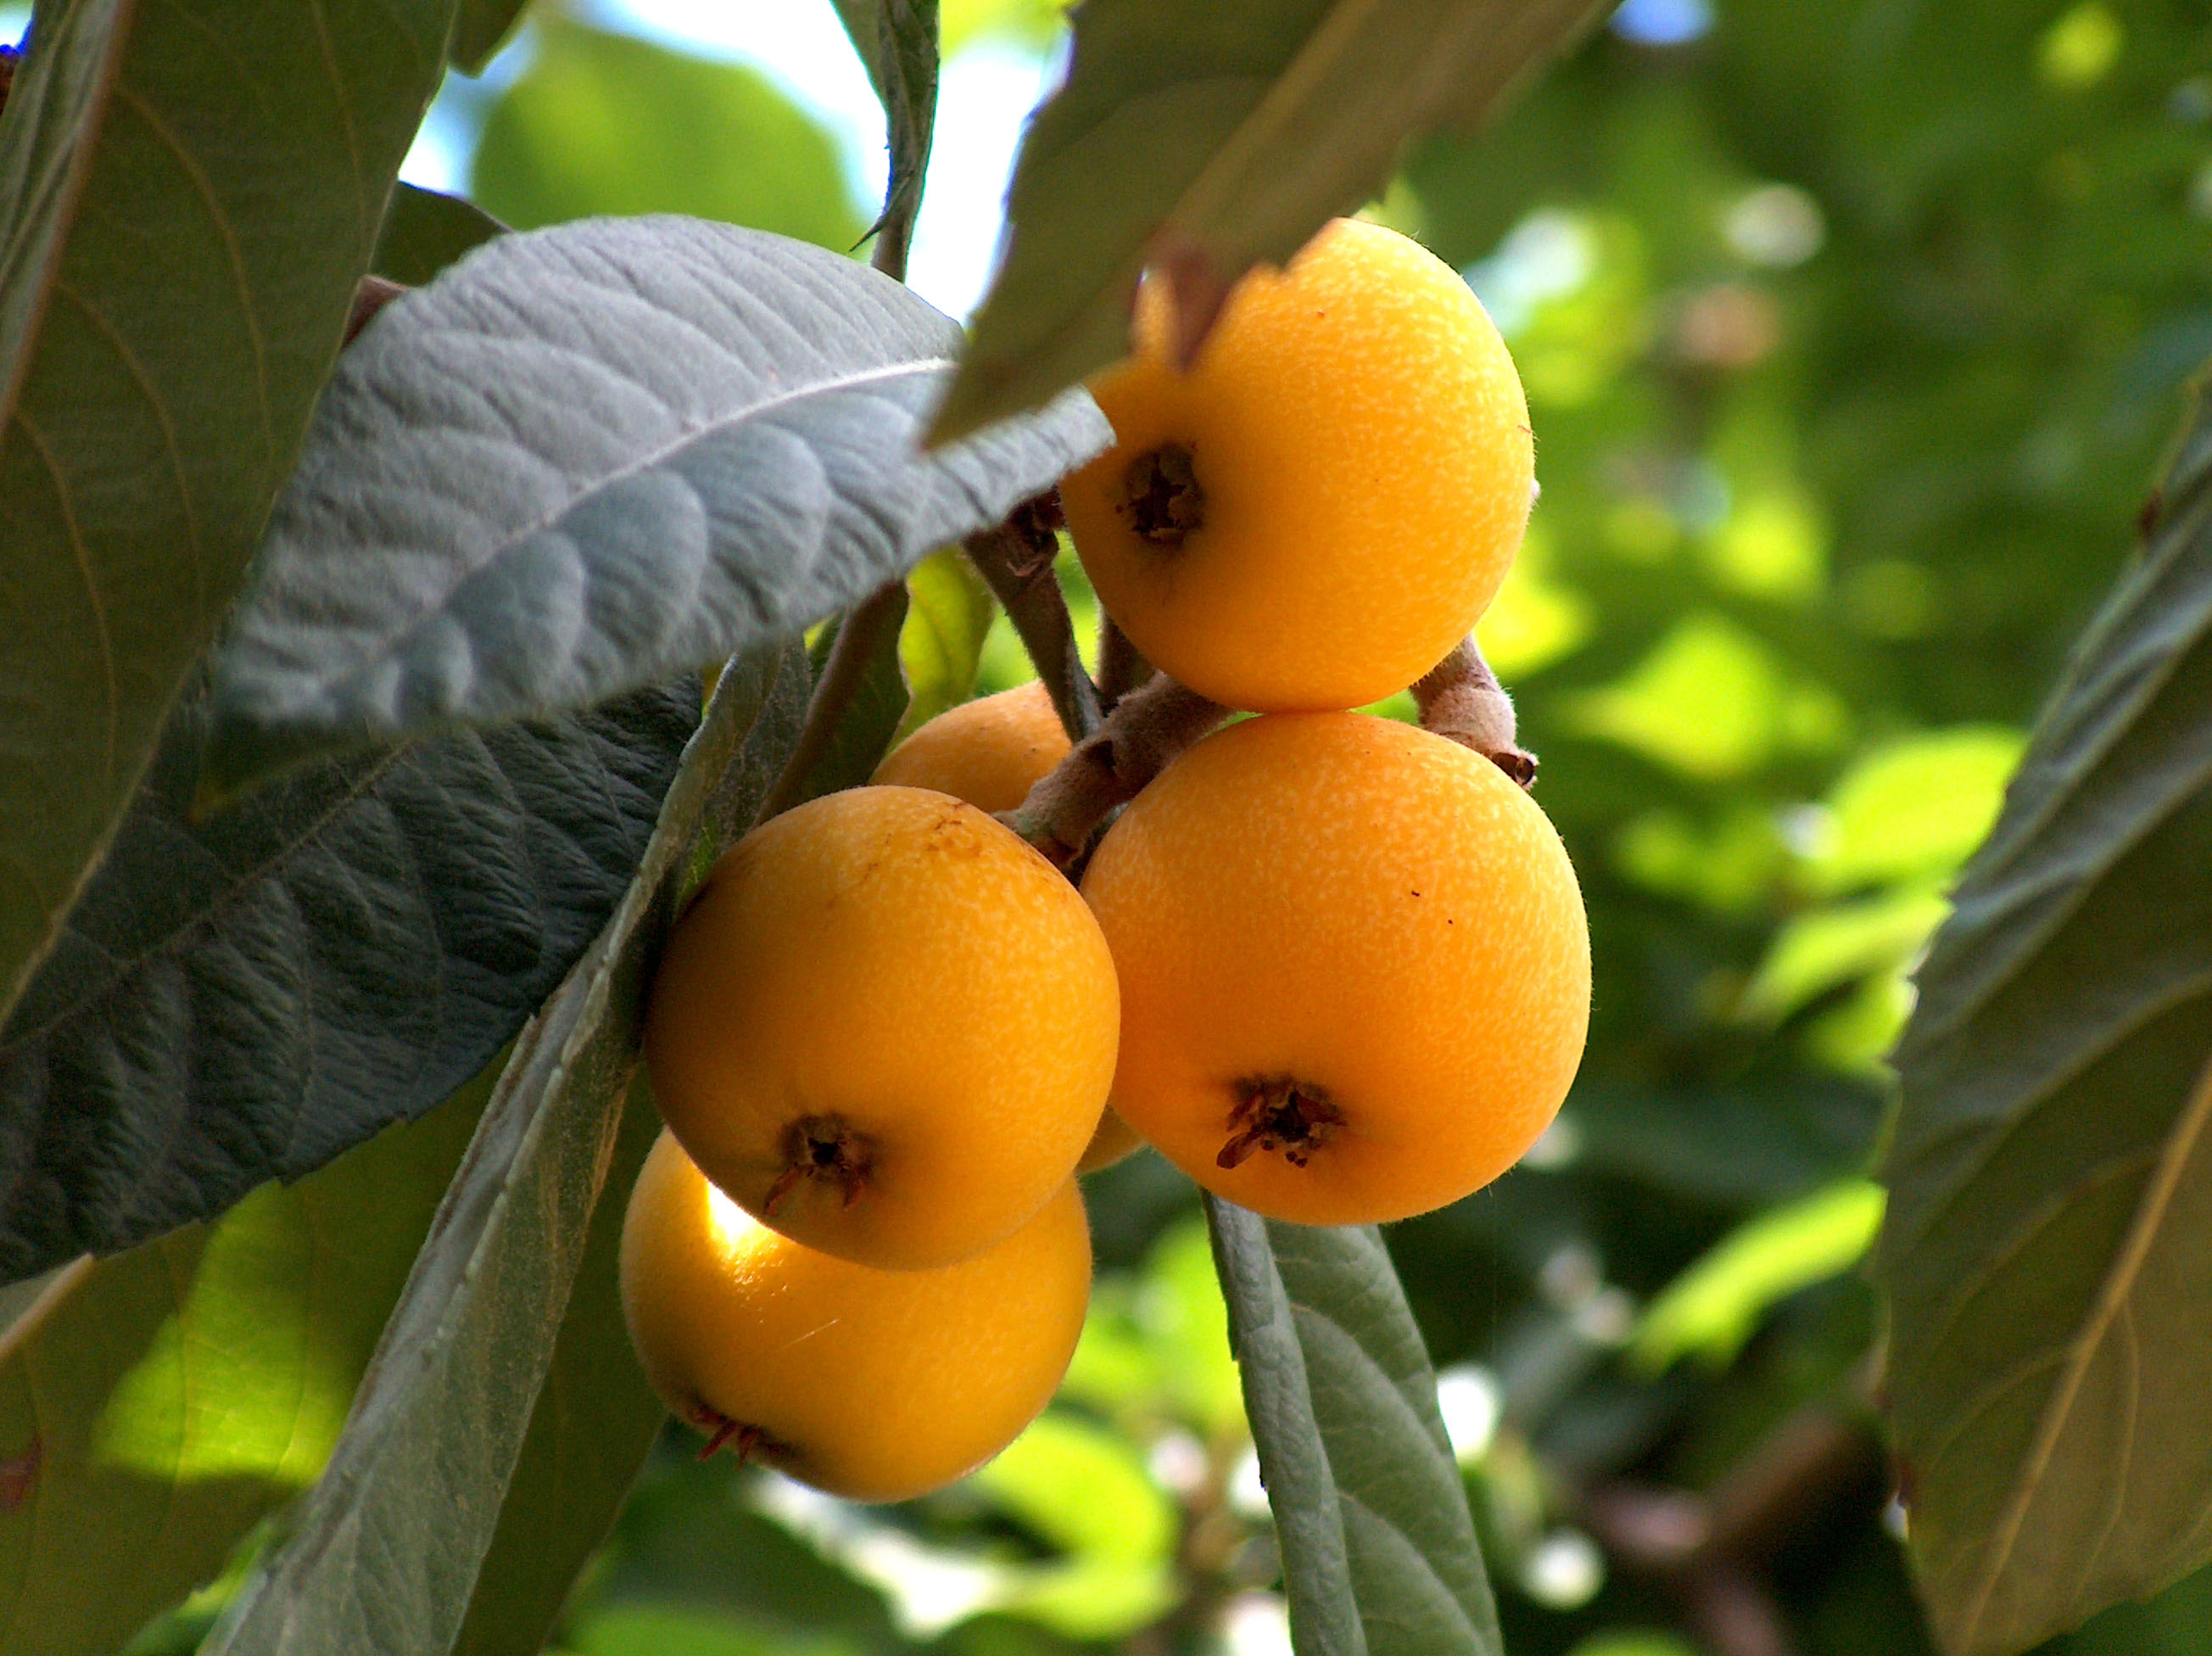
\includegraphics[width=\textwidth]{nispero.jpg}
(photo from http://malagasecome.es/)
}

%----------------------------------------------------------------------------------------
%	RESULTS 2
%----------------------------------------------------------------------------------------

\headerbox{Components}{name=components,column=1,below=architecture}{ % This block's bottom aligns with the bottom of the conclusion block
\begin{itemize}\compresslist
  \item a console instance that tracks at any moment the status of the whole 
system giving the user the opportunity to check at any point the 
current status of the computations, workers, etc
  \item a manager instance that is in charge of deploying and undeploying 
the group of workers
  \item a set of workers that performs the computations/tasks in a parallel, 
independent way 
  \item SQS queues for input, output and error messages
  \item S3 objects for input and output files 
\end{itemize}


}

\headerbox{Console}{name=console,column=2,below=architecture,bottomaligned=components}{ % This block's bottom aligns with the bottom of the conclusion block

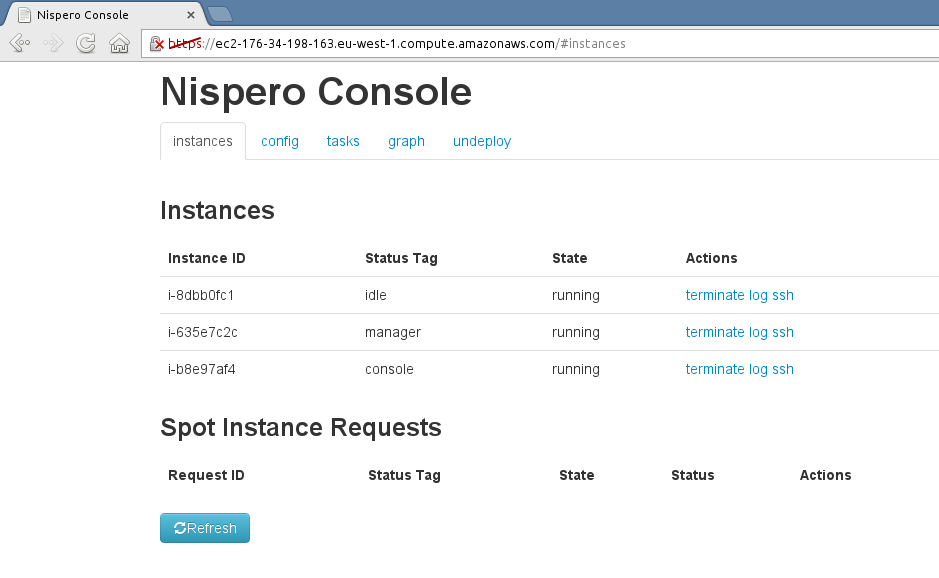
\includegraphics[width=\textwidth]{console.png}

}
%----------------------------------------------------------------------------------------

\headerbox{Monoids}{name=monoids,span=2,column=1,below=components}{ % This block is as tall as the references block

$$ Reads \otimes Reads \xrightarrow{merge} Reads \xrightarrow{BLAST} AssignTable \otimes Reads $$



We are using idempotent commutative monoids to describe distributed	systems in Nispero. They are:

\begin{itemize}\compresslist
  \item powerful enough to build complex system
  \item easy to work with them abstractly (graphical workflow editor that produces distributed systems).
\end{itemize}

}


\end{poster}

\end{document}